\begin{frame}{Distribution of Track Parameters}
    % \centering
    \textbf{Basic Plot Parameters to assess}
    \begin{itemize}
        \item longTracks
        % \item Track Propagation Error [SKIP]
        \item Track Chi2
        \item Track Chi2perDoF
        \item Track nDoF
        \item Track charge
        \item Track nLayers
    \end{itemize}
\end{frame}

\begin{frame}{Distribution of longTracks}    
    \begin{figure}        
        % 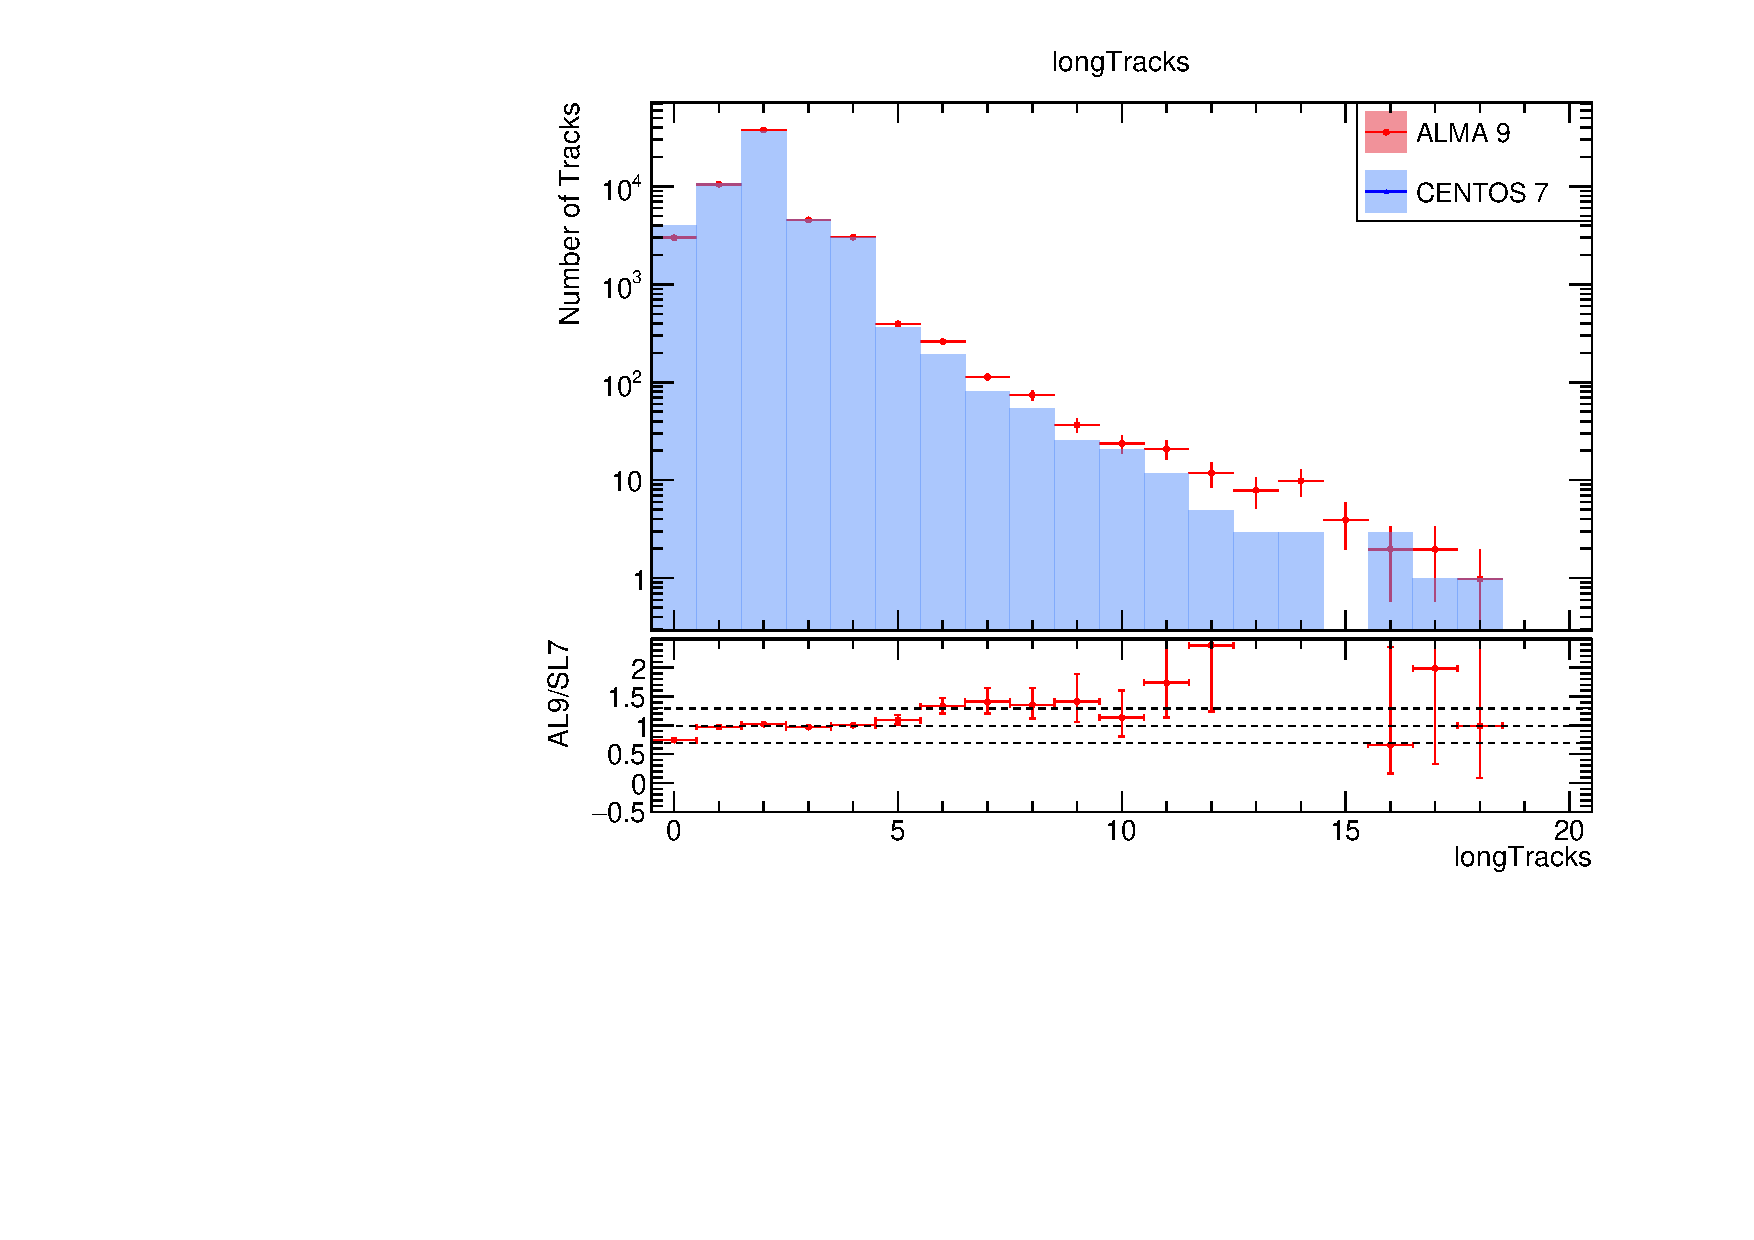
\includegraphics[width=\linewidth]{./output/longTracks.pdf}
        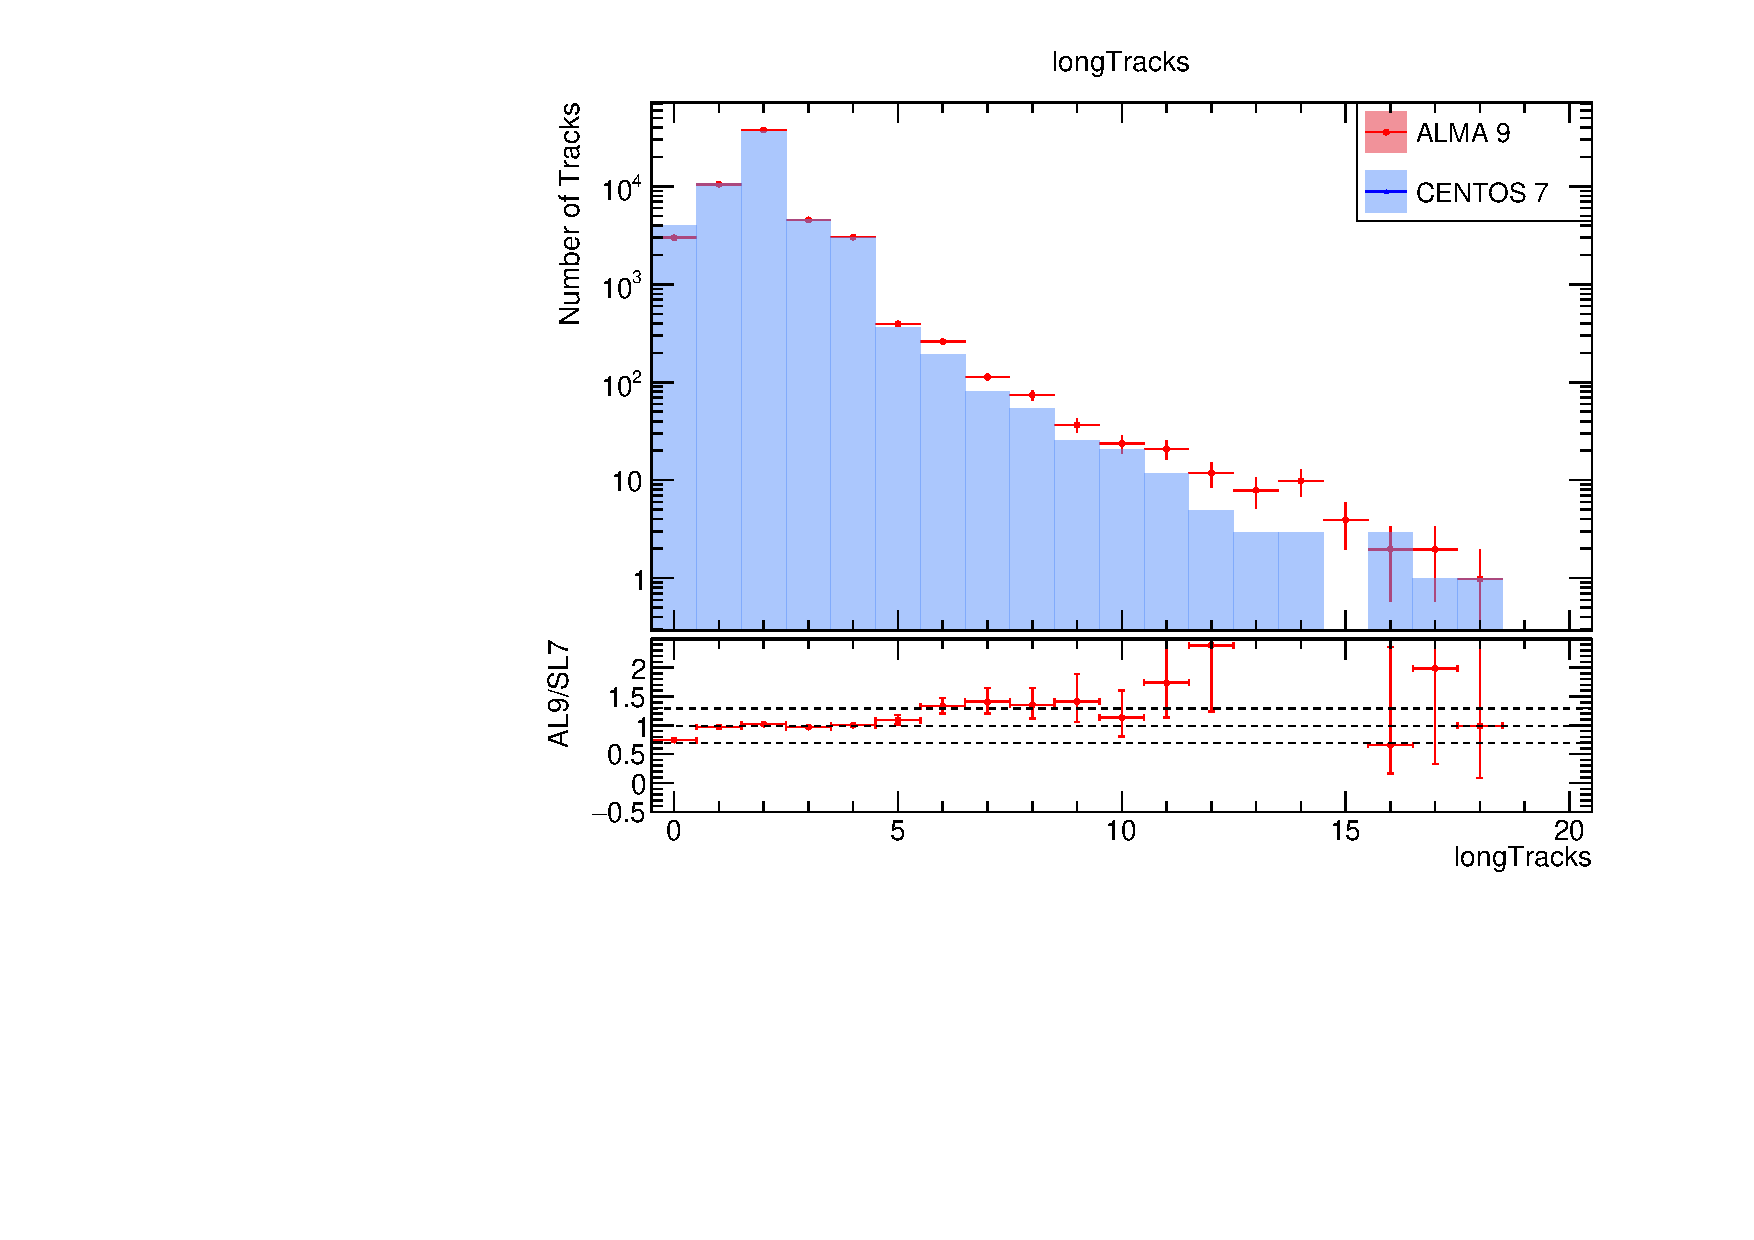
\includegraphics[width=0.8\linewidth]{output/longTracks.pdf}
    \end{figure}
    \vspace{-0.5cm}
    \begin{itemize}
        % \item Overall agreement is strong, especially in the early bins.
        \item \small ALMA9 has fewer 0-track events;
        \item \small Also reconstructs more events with more than 5 tracks.
        \item \small Total number of longTracks: CENTOS7: 115,206, AL9: 118,491
        \item \small A 2.8\% increase in longTracks in AL9.
        % \item longTracks \>5 shows more discrepancy, Concerning?
    \end{itemize}
\end{frame}


% \begin{frame}{Distribution of TrackPropagationError [SKIP]}
%     \begin{figure}
%         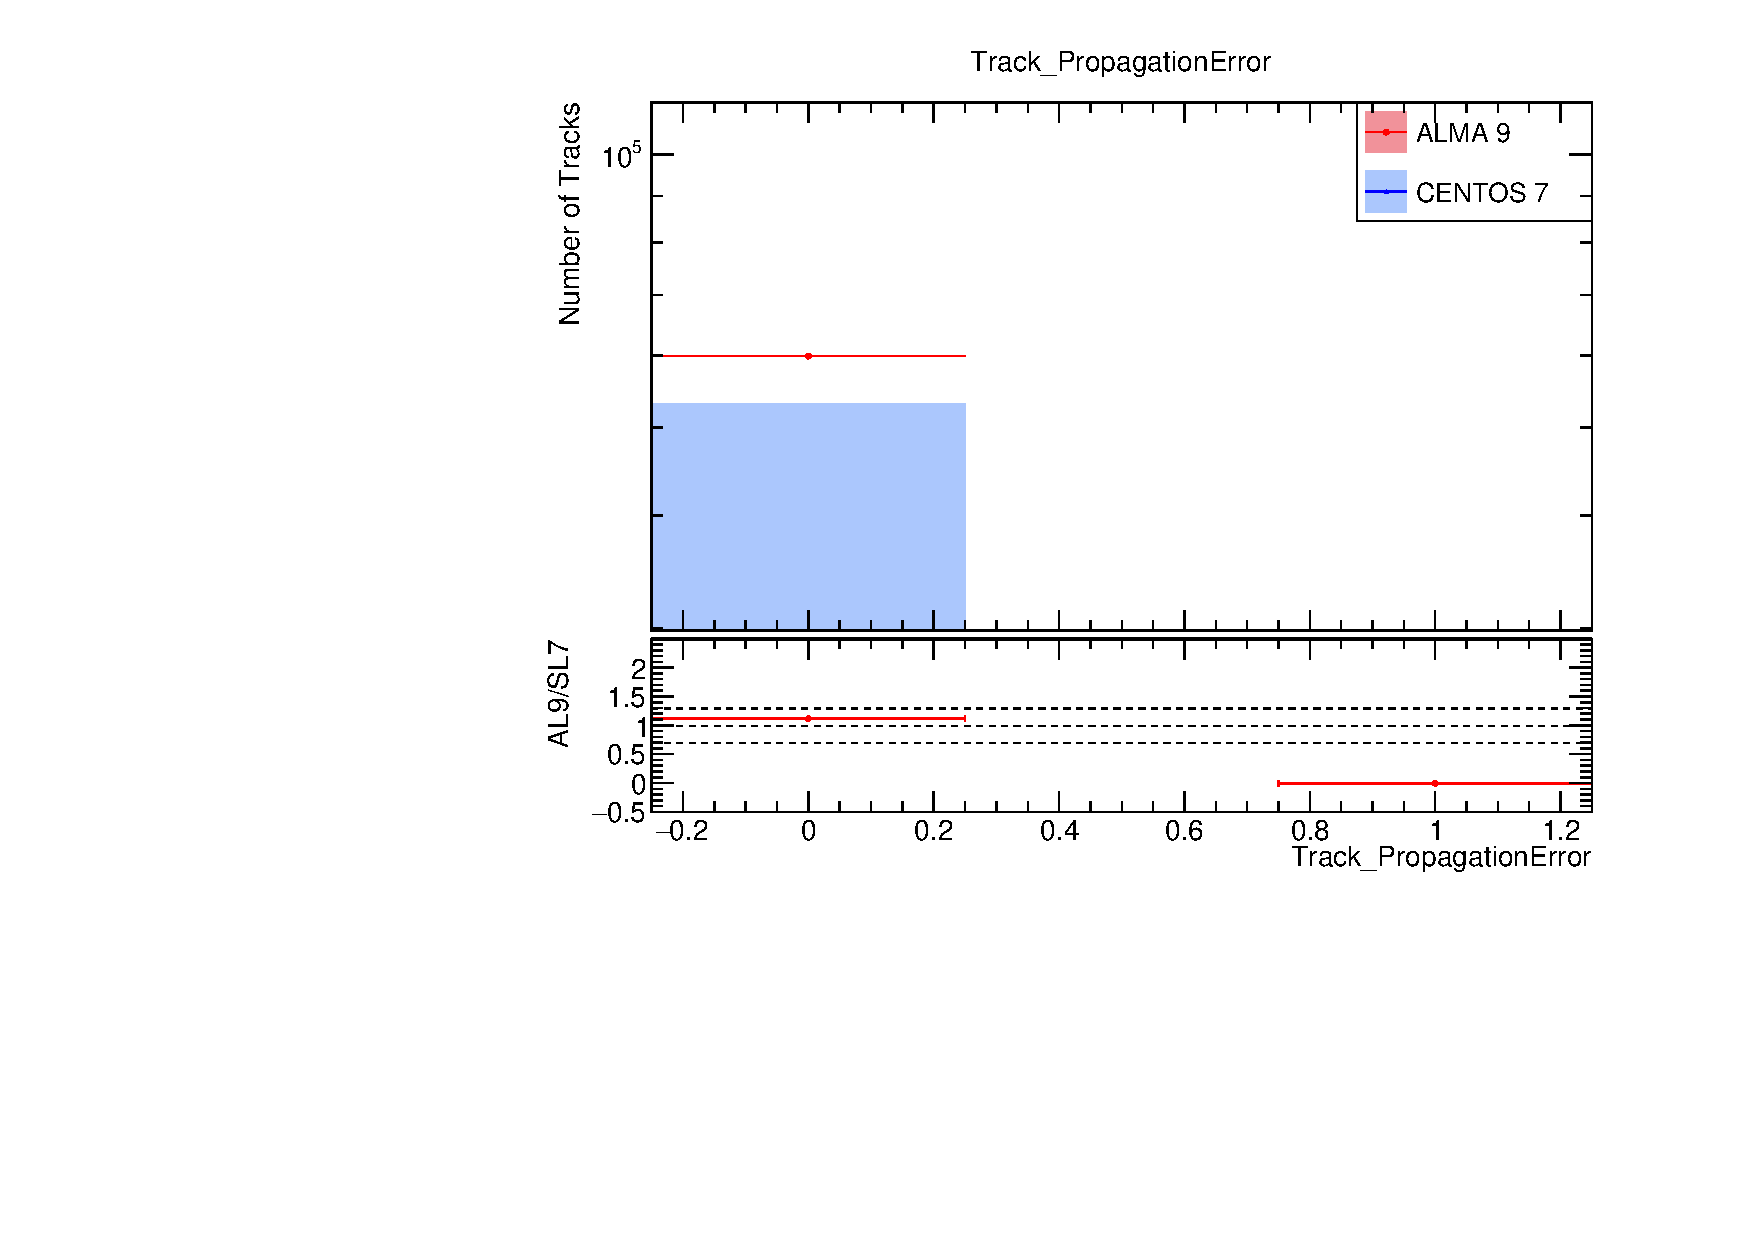
\includegraphics[width=0.9\linewidth]{output/Track_PropagationError.pdf}
%     \end{figure}
%     \vspace{-0.5cm}
%     \begin{itemize}
%         \item More TrackPropagationErrors in CENTOS7.
%     \end{itemize}
% \end{frame}

\begin{frame}{Distribution of TrackChi2}
    \begin{figure}
        \begin{subfigure}{0.49\linewidth}
            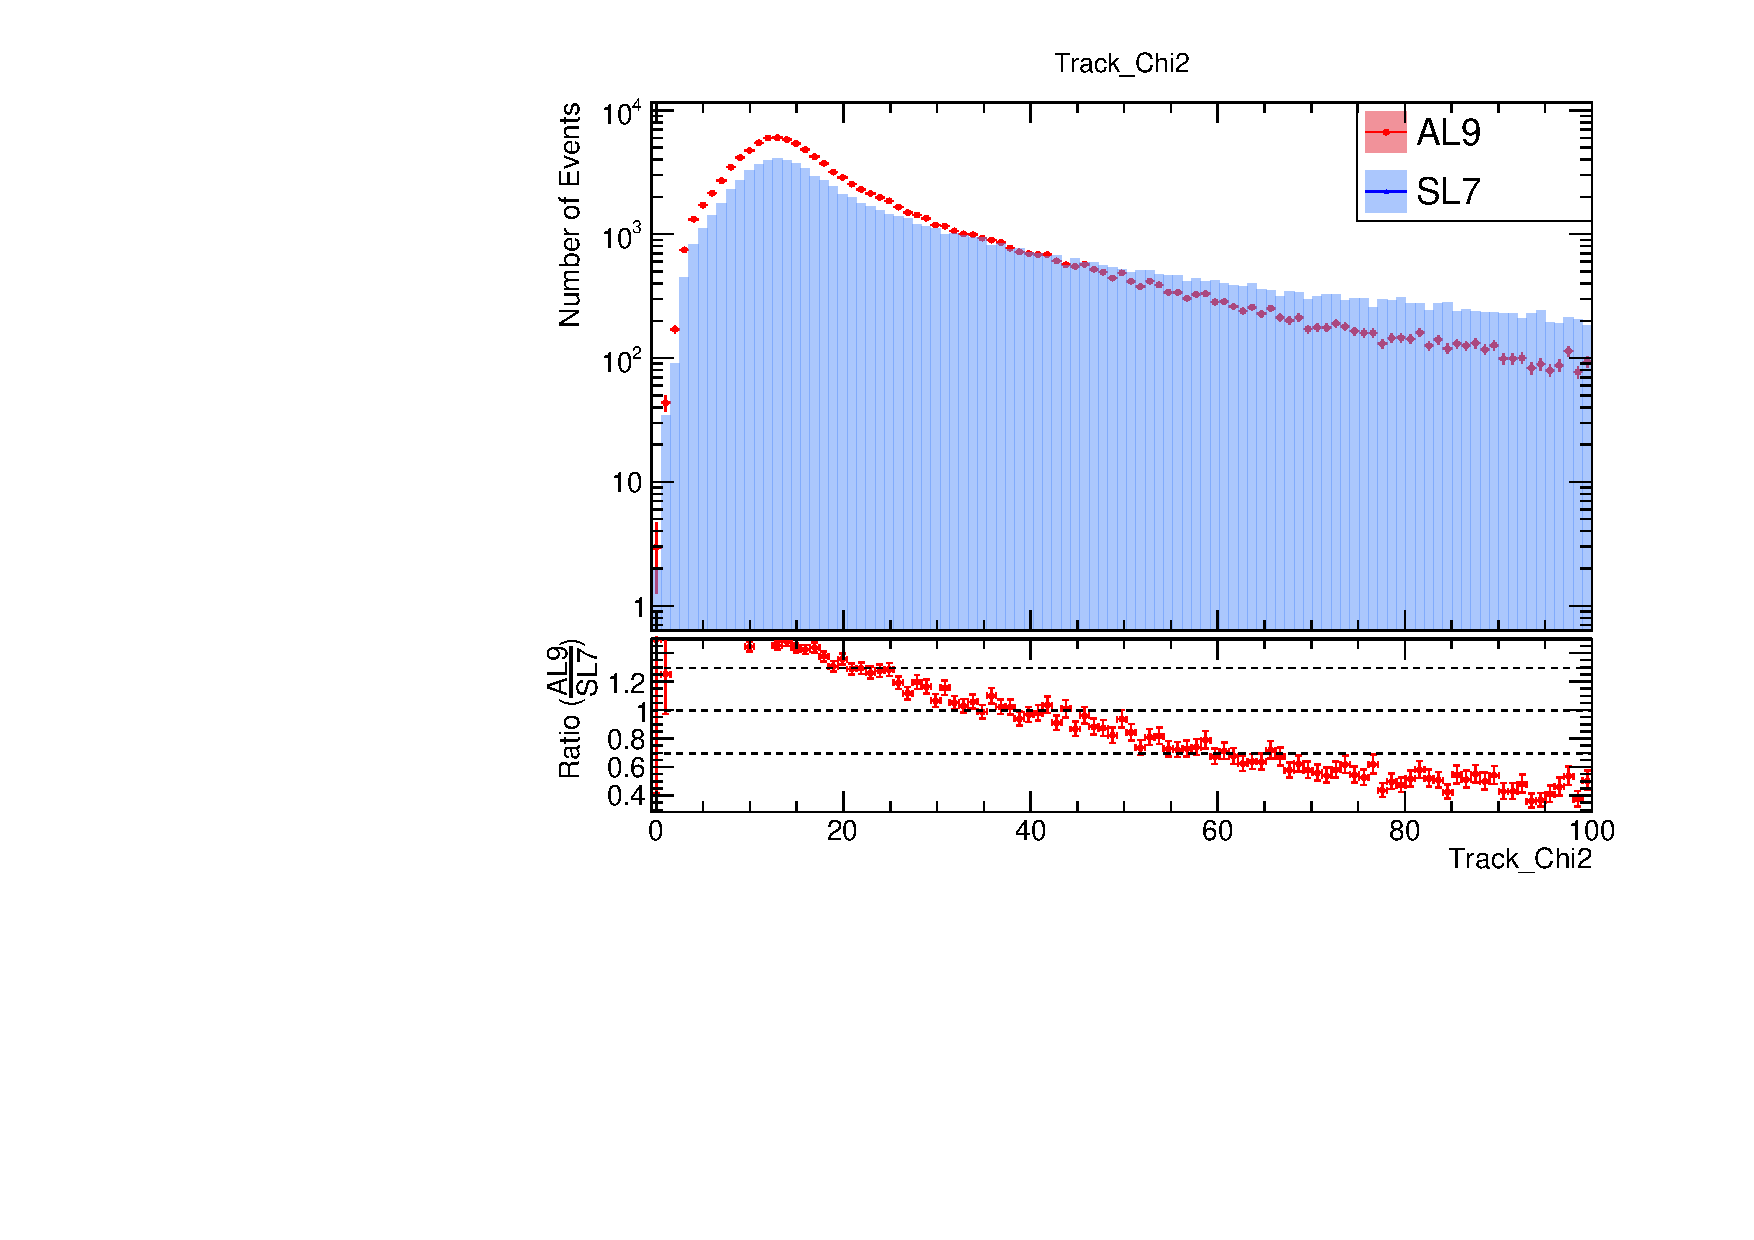
\includegraphics[width=\linewidth]{./output/Track_Chi2.pdf}
        \end{subfigure}
        \begin{subfigure}{0.49\linewidth}
            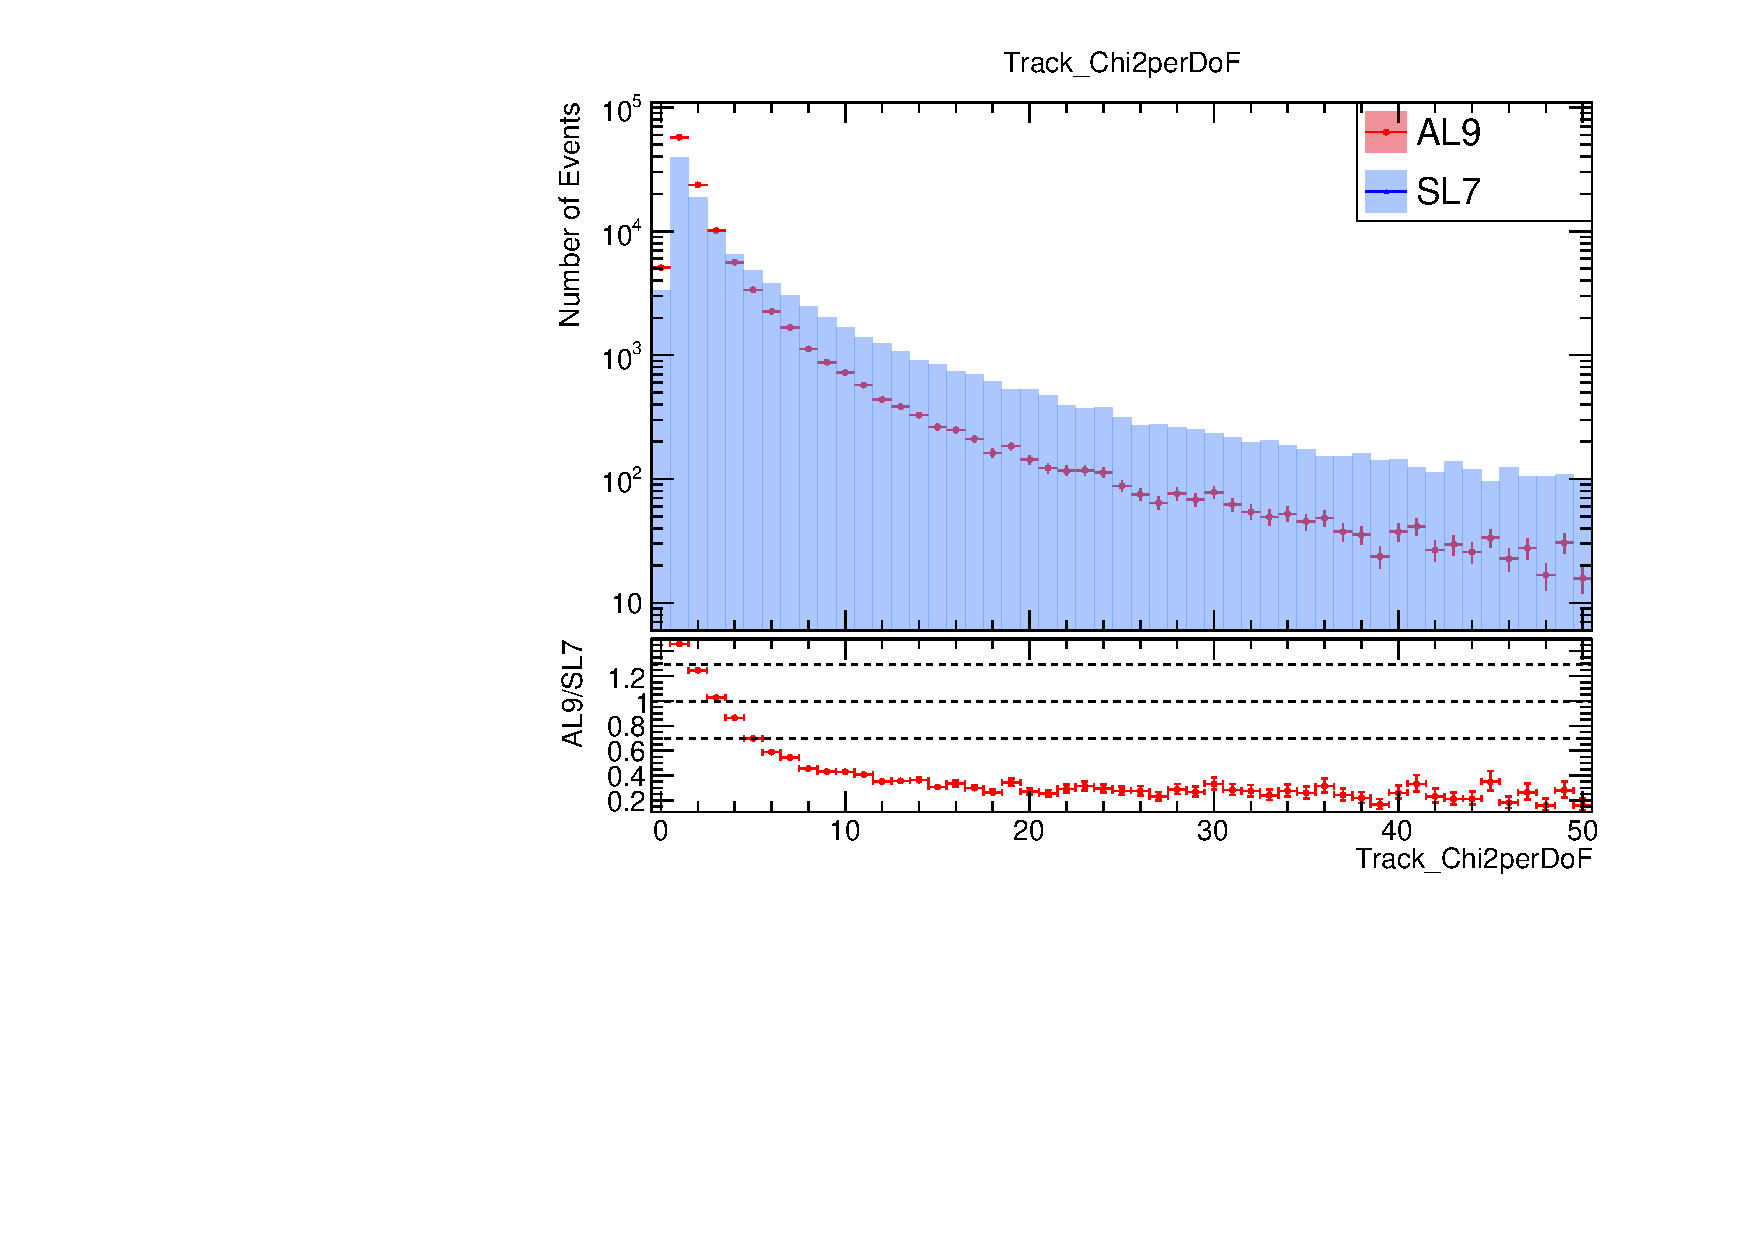
\includegraphics[width=\linewidth]{./output/Track_Chi2perDoF.pdf}
        \end{subfigure}
        \begin{itemize}
            \item Displays the greatest improvement in ALMA9.
            \item Overall Tracks have lower Chi2/DoF in ALMA9.
        \end{itemize}
    \end{figure}
\end{frame}

% \begin{frame}{Distribution of TrackChi2perDoF}
%     \begin{figure}
%         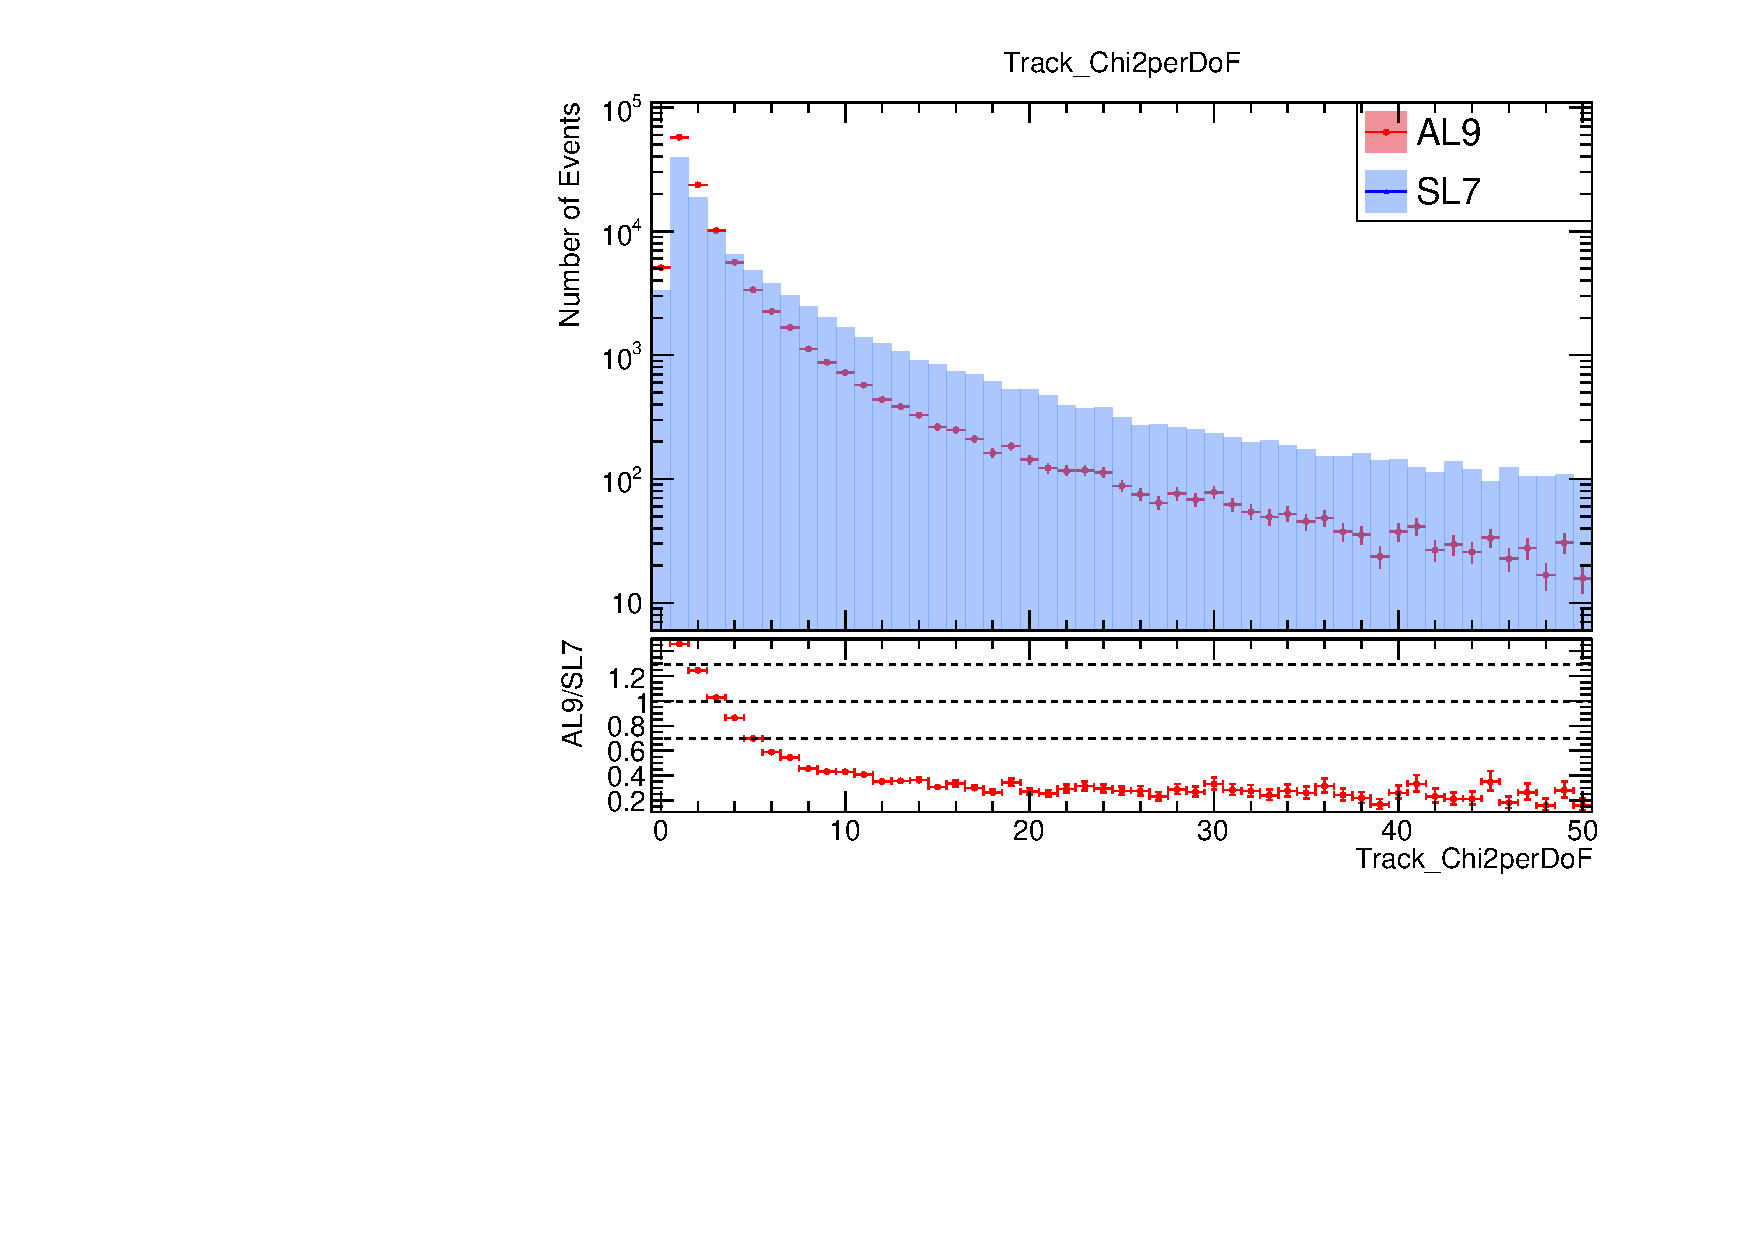
\includegraphics[width=0.9\linewidth]{./output/Track_Chi2perDoF.pdf}
%     \end{figure}
%     \vspace{-0.5cm}

% \end{frame}

\begin{frame}{Distribution of TrackNDoF}
    \vspace{-0.3cm}
    \begin{figure}
        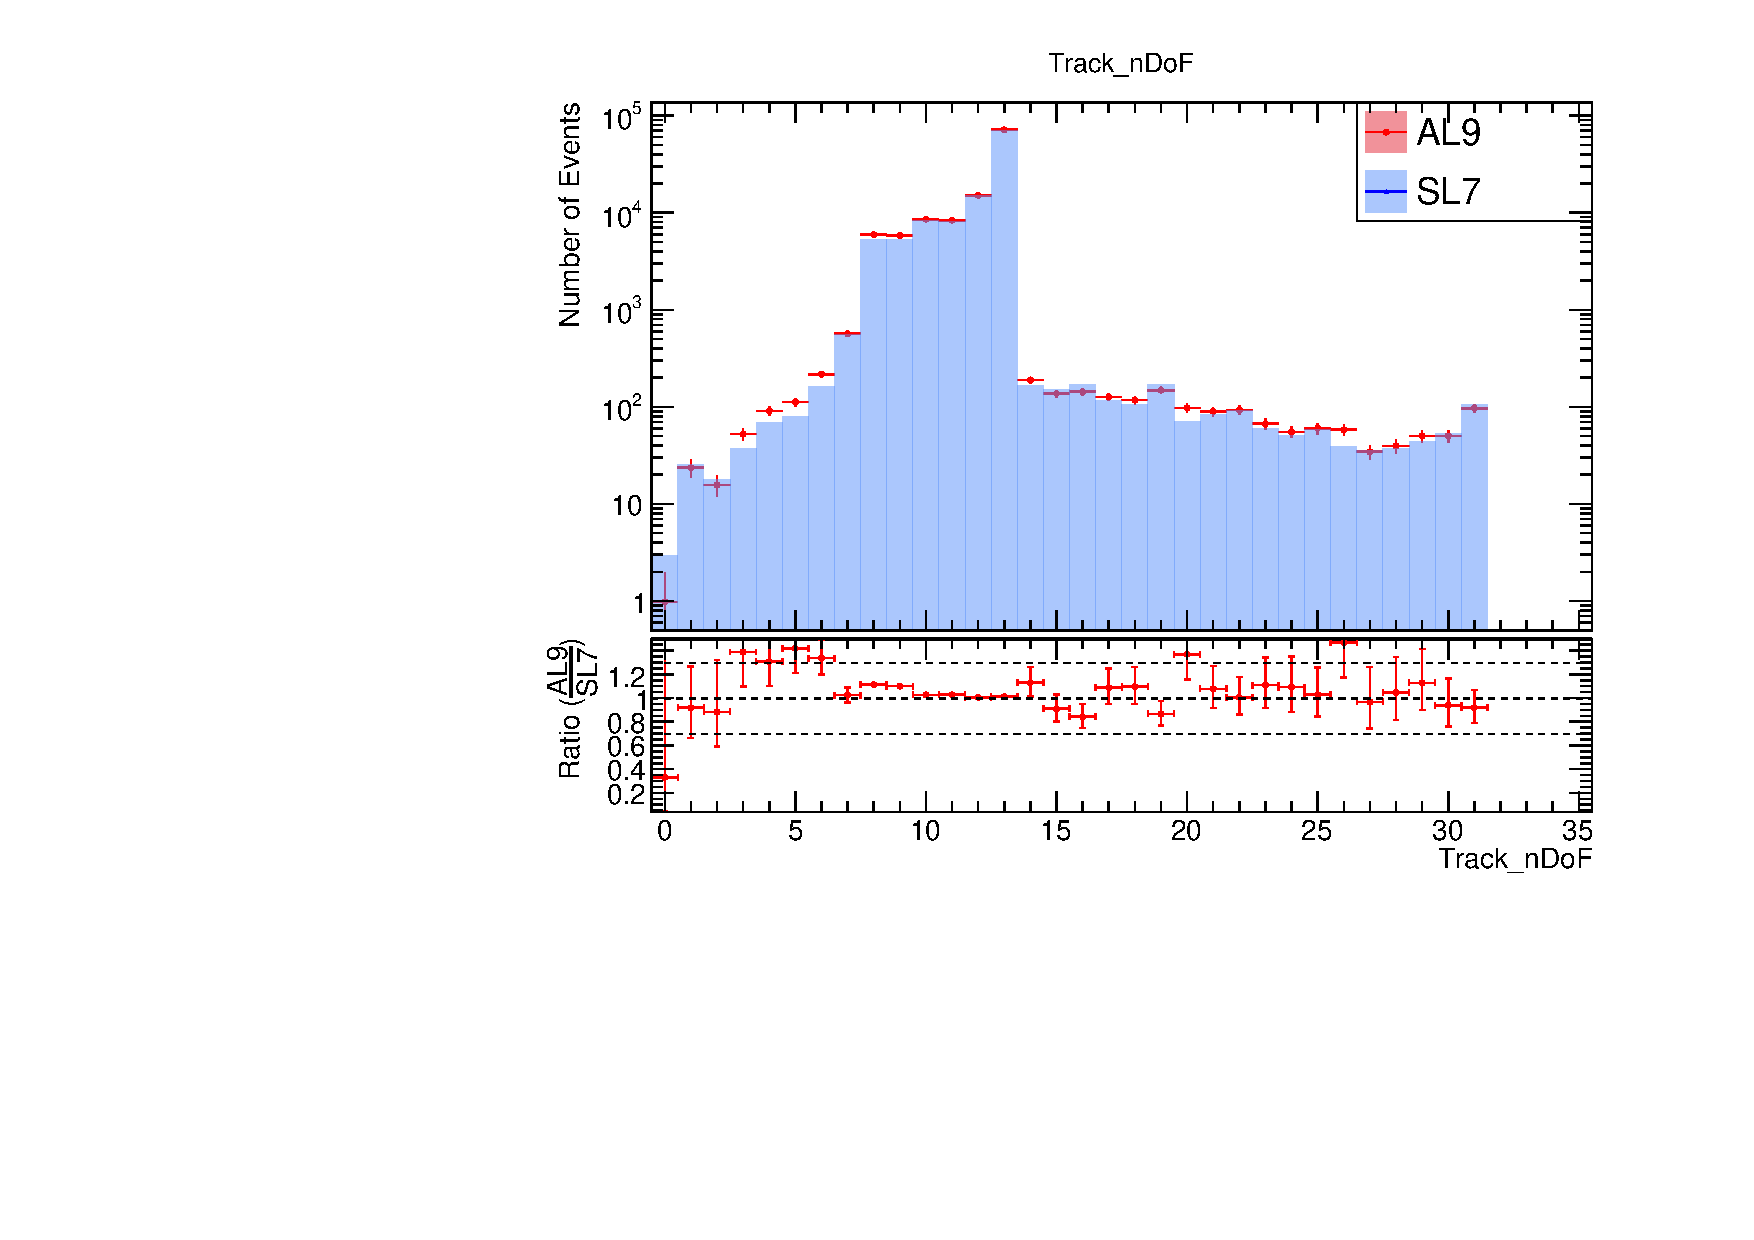
\includegraphics[width=\linewidth]{./output/Track_nDoF.pdf}
    \end{figure}
    \vspace{-0.65cm}
    \begin{itemize}
        \item Generally strong agreement, except for bins 3-5.
    \end{itemize}
\end{frame}

\begin{frame}{Distribution of Track Charge}
    \vspace{-0.3cm}
    \begin{figure}
        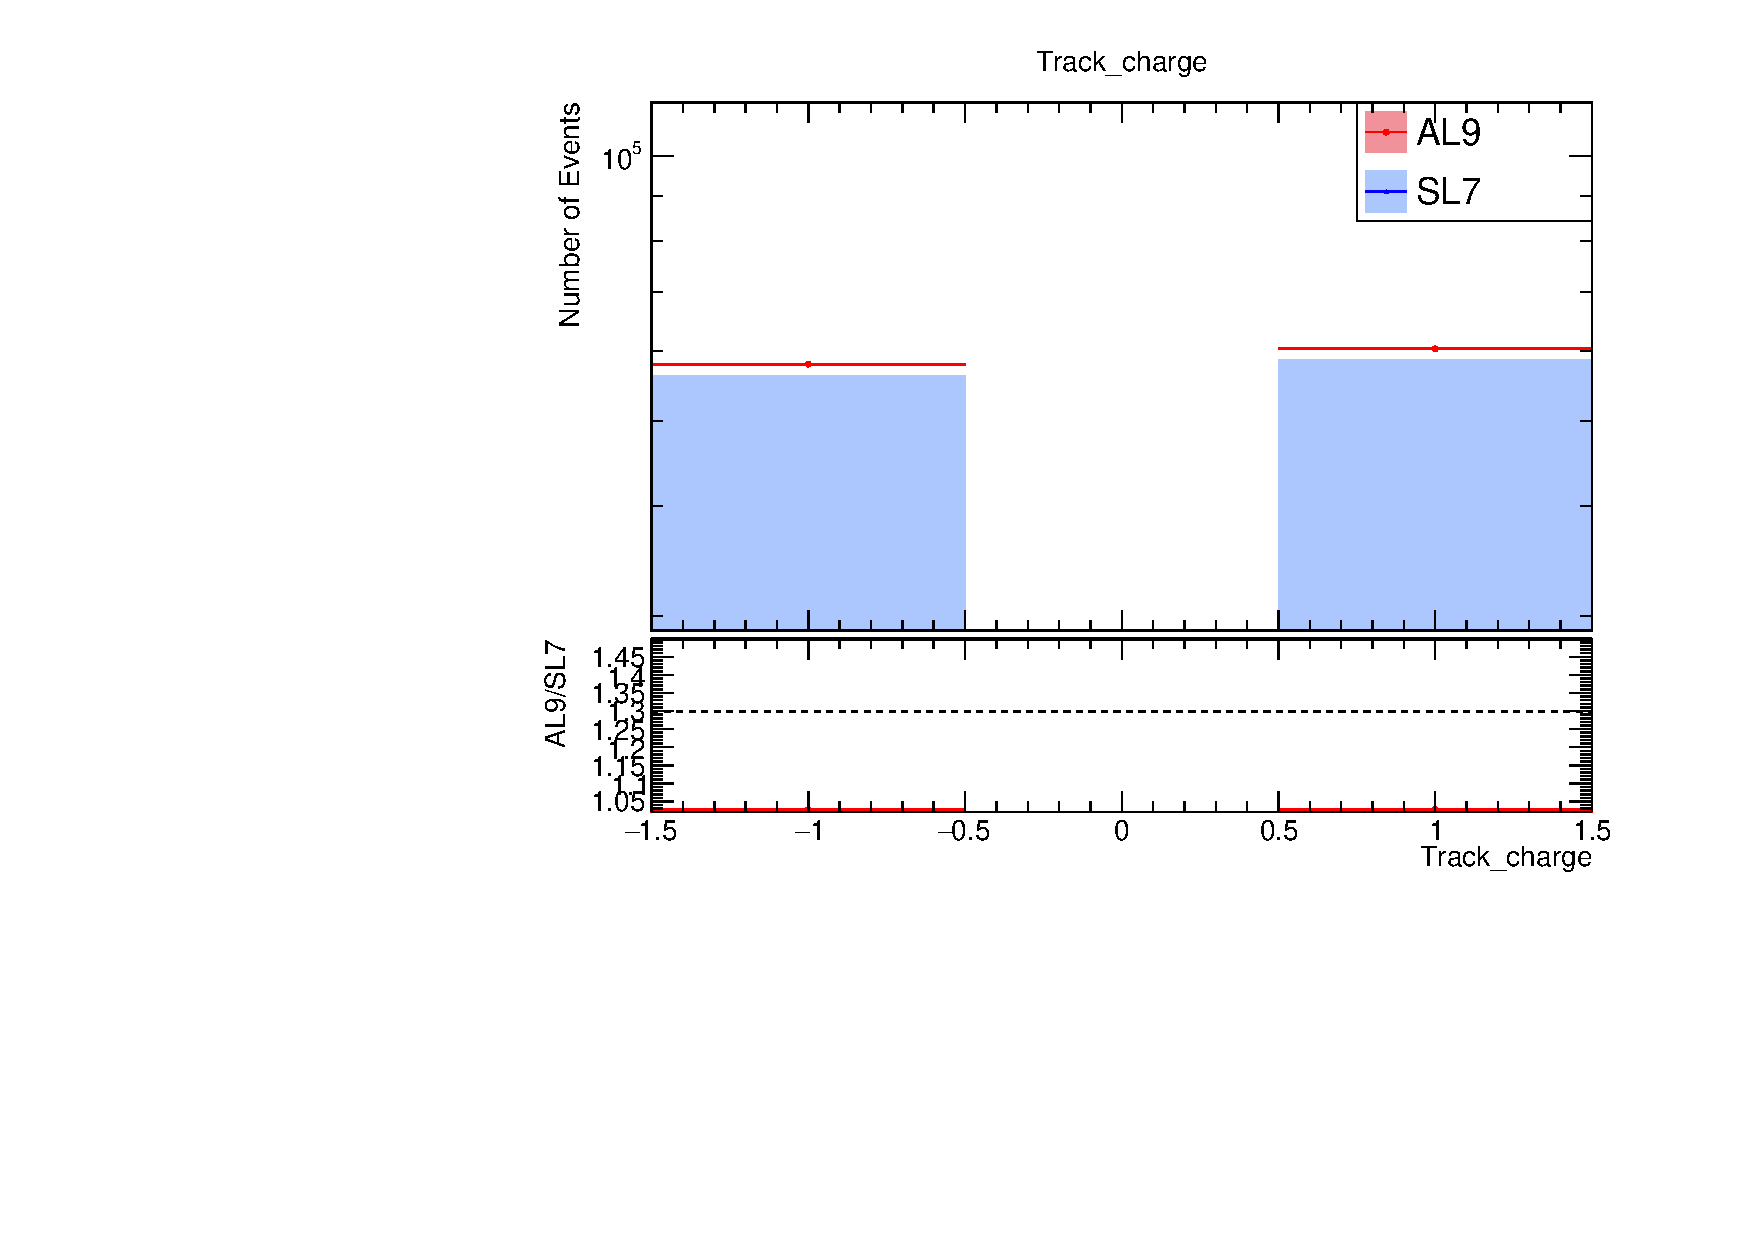
\includegraphics[width=0.9\linewidth]{./output/Track_charge.pdf}
    \end{figure}
    \vspace{-0.6cm}
        \begin{itemize}
            \small
            \item The ratio is 1.028 [same factor of increase seen in longTracks]
            \item Ratio of positive to negative tracks is 1.04 in both. ChargeMISID?
        \end{itemize}
\end{frame}

\begin{frame}{Distribution of Track nLayers}
    \vspace{-0.3cm}
    \begin{figure}
        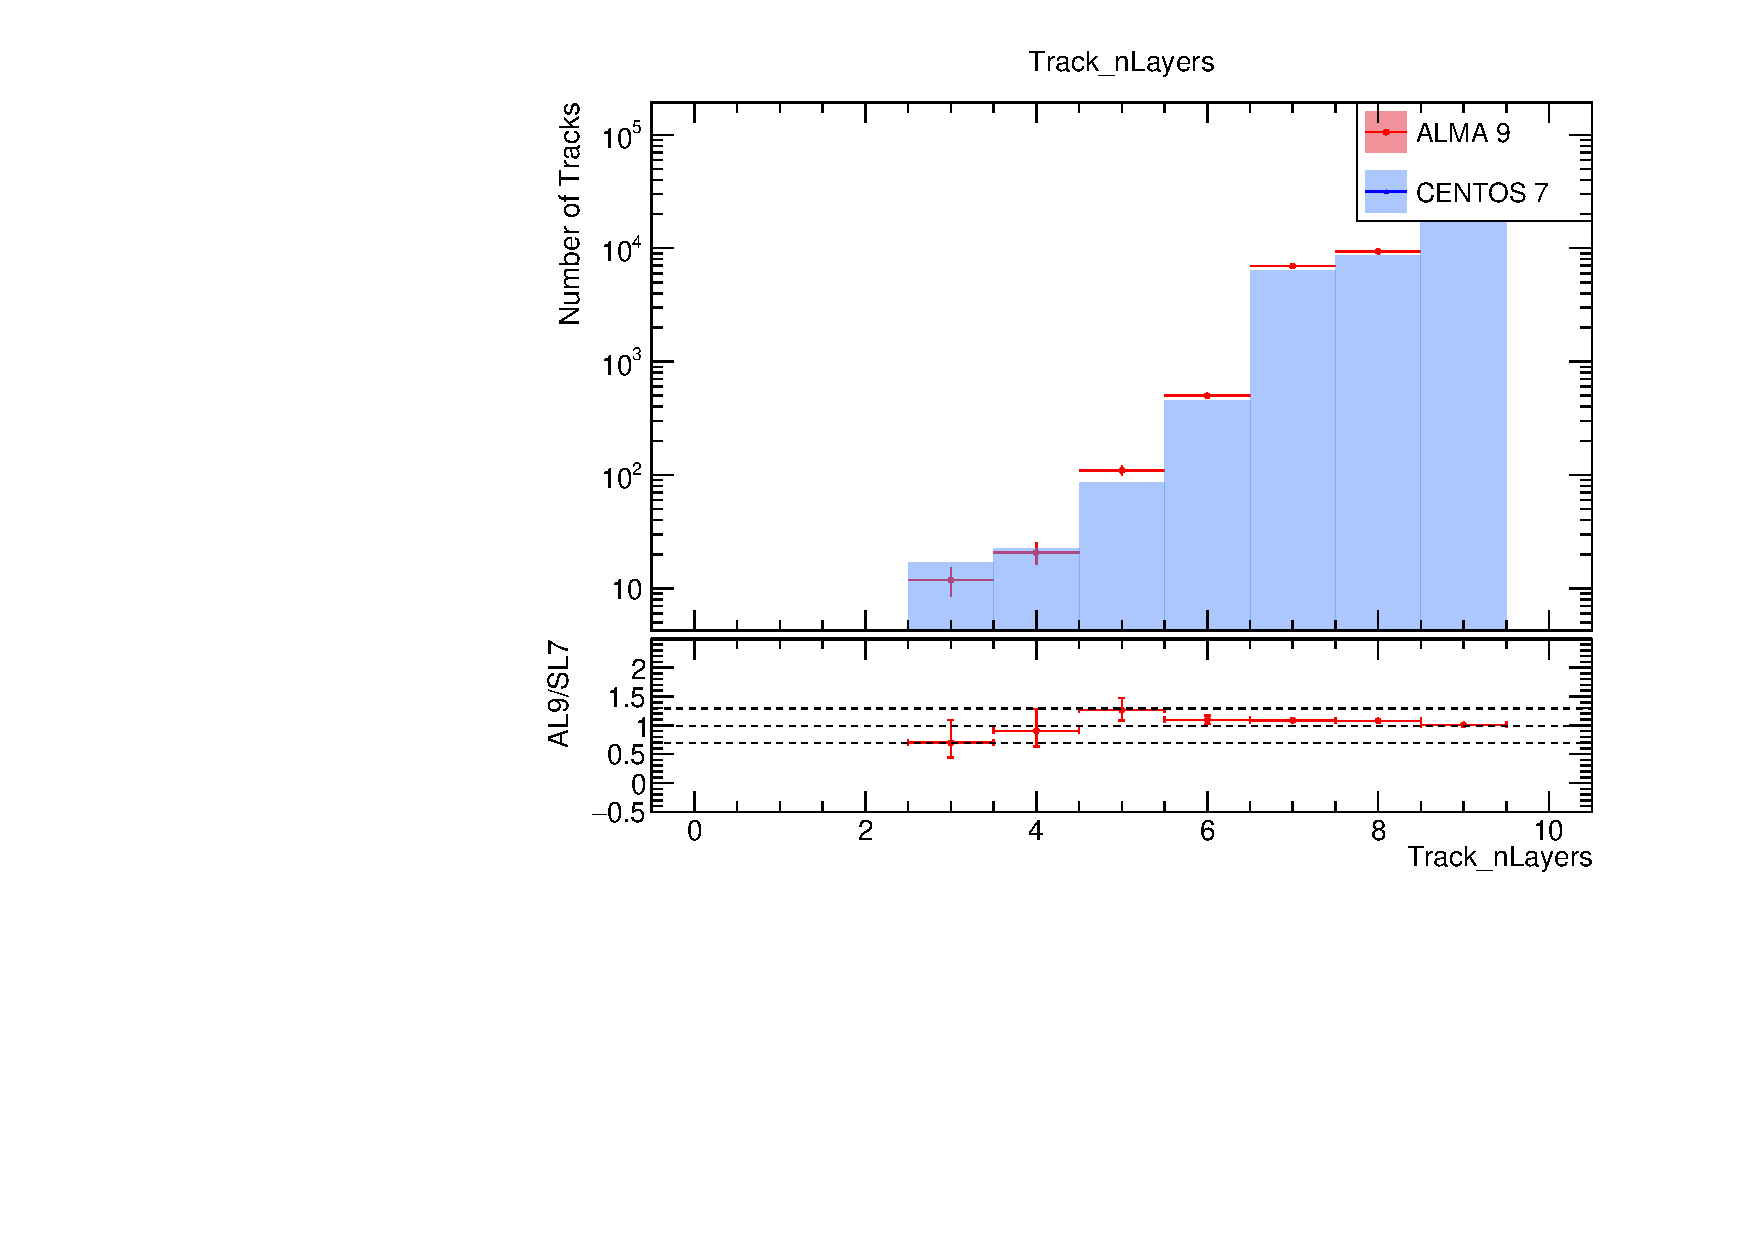
\includegraphics[width=0.95\linewidth]{./output/Track_nLayers.pdf}
    \end{figure}
    \vspace{-0.6cm}
    \begin{itemize}
        \item Similar agreement within statistical uncertainties.
    \end{itemize}
\end{frame}

% \begin{frame}{Comments on Track Parameters}
%     \begin{itemize}
%         \item longTracks \> 5 is a mess, But not particularly useful
%         \item Track Propagation Error is a easily interpretable function
%         \item Track Chi2 changed a lot, much higher peak and lower tail in AL9, which is good.
%         \item TrackNDoF shows good agreement except betweeen 3-5
%         \item Track Charge in AL9 is slightly elevated, not sure why
%         \item Track nLayers is also decent agreement except at 5-8
%     \end{itemize}
% \end{frame}